%
%  Vincent Yannello
%
\documentclass[12pt,fullpage]{article}
\usepackage{fullpage}
\usepackage{amsmath}
\DeclareMathOperator{\erf}{erf}
\usepackage{psfrag}                                          % LaTeX graphics tool
\usepackage{pslatex}                                         % avoids the default cmr font
\usepackage{graphicx}                                        % graphics package 
\usepackage{epsfig}                                          % figures
\usepackage{hyperref}
\usepackage{color}

\begin{document}

\noindent
{\bf Arcsin distribution} (from \color{blue}\url{http://www.math.wm.edu/~leemis/chart/UDR/UDR.html}\color{black})

\noindent
The shorthand $X \sim {\rm arcsin}$ is used to indicate that the
random variable $X$ has the arcsin distribution.
An arcsin random variable $X$ has probability density function 
$$
f(x) = {\frac {1}{\pi \,\sqrt {x \left( 1-x \right) }}}
 \quad \quad 0<x<1.
$$
The probability density function is illustrated below.
{\begin{figure}[h!]
\begin{center}
\psfrag{labx}{$x$}
\psfrag{labf}{$f(x)$}
\includegraphics[width=3.2in]{ArcsinPlot.ps}
\end{center}
\end{figure}}\\
The cumulative distribution on the support of X is
$$
F(x) = P(X \leq x) = \frac{\pi + 2\arcsin(2x-1)}{2\pi} \quad \quad 0<x<1.
$$
The survivor function on the support of X is
$$
S(x) = P(X \geq x) = \frac{\pi - 2\arcsin(2x-1)}{2\pi} \quad \quad 0<x<1.
$$
The hazard function on the support of X is
$$
h(x)=\frac{f(x)}{S(x)}= \frac{2}{\sqrt{x(1-x)}(\pi - 2\arcsin(2x-1))}\quad \quad 0<x<1.
$$
The inverse distribution function of X is
$$
F^{-1}(u)= \frac{1}{2} -\frac{1}{2}\cos(\pi \kern 0.08 em u) \quad \quad 0 < u < 1.
$$
The cumulative hazard function, moment generating function, and characteristic function
on the support of $X$ are mathematically intractable.\\
\\
\noindent
The population mean, variance, skewness, and kurtosis of $X$ are
$$
E[X] =\frac{1}{2} \qquad \qquad 
V[X] = \frac{1}{8} \qquad \qquad 
E\left[ \left( \frac{X - \mu}{\sigma} \right) ^ 3 \right] = 0 \qquad \qquad 
E\left[ \left( \frac{X - \mu}{\sigma} \right) ^ 4 \right] = -\frac{3}{2}.
$$

\vspace{0.1in}

\noindent
{\bf APPL verification:}
The APPL statements
\begin{verbatim}
X := [[x -> 1 / (Pi * sqrt(x * (1 - x)))], [0, 1], ["Continuous", "PDF"]];
CDF(X);
SF(X);
HF(X);
IDF(X);
Mean(X);
Variance(X);
Skewness(X);
Kurtosis(X);
MGF(X);
\end{verbatim}
verify the cumulative distribution function, survivor function, hazard function, inverse distribution function, population mean, variance, skewness, kurtosis, and moment generating function.

\end{document}
